\documentclass[conference]{IEEEtran}
% \IEEEoverridecommandlockouts
% The preceding line is only needed to identify funding in the first footnote. If that is unneeded, please comment it out.
\usepackage{cite}
\usepackage{amsmath,amssymb,amsfonts}
\usepackage{algorithmic}
\usepackage{graphicx}
\usepackage{textcomp}
\usepackage{xcolor}
\usepackage{hyperref}

\def\BibTeX{{\rm B\kern-.05em{\sc i\kern-.025em b}\kern-.08em

T\kern-.1667em\lower.7ex\hbox{E}\kern-.125emX}}
\begin{document}

\title{Reinforcement Learning on Unity Machine Learning Agents Toolkit}

\author{\IEEEauthorblockN{\textbf{Hong Jing Khok}}
School of Computer Science and Engineering, Nanyang Technological University, Singapore
}

\maketitle

\begin{abstract}
This is a report for an assignment for the course, Artificial Intelligence in Game Design (DM6127). This report will describe the mechanics of the game and its design and present the thought process of designing a reinforcement learning agent capable of playing this game. We explore scenarios on various difficulties and compare our agent's performance. Iteratively, we developed and evaluated each hypothesis; and recorded its results. The source code and videos of the gameplay are available on a companion website.
\end{abstract}

\begin{IEEEkeywords}
Reinforcement Learning, Unity
\end{IEEEkeywords}

\section{Introduction}

Unity is a popular game creation platform where users can build 3D games and simulations. With the rise in popularity in reinforcement learning algorithms, Unity Technologies introduced the Unity Machine Learning Agents Toolkit to allow users to utilize machine learning technologies on Unity. This enables machine learning researchers to have a realistic environment and training scenarios, and game developers can build interesting game AI.

Our goal is to build a turret game where the player can shoot enemy units while allowing friendly units to enter. We will train a reinforcement learning agent to play as the turret, where its goal is to allow ten friendly units to enter the base, and loses if an enemy unit has entered the base or if two friendly units were shot.

\section{Game Mechanics}

\subsection{Components}

There are three main components in this game, 1) \textit{game controller}, 2) \textit{turret}, and 3) \textit{unit}.

The game controller is responsible for spawning units and managing game states. The \textit{Update} function will keep track of last spawn units and spawn units according to the set time interval. Then, it will check each unit in the game scene for its state. For units in state \textit{isHit} or \textit{isSaved}, the game controller will increase the respective counters accordingly. These counters are critical to determine the win and lose conditions. For units that are alive, the game controller will execute a move order for units to move units closer to the turret. The units will turn to face the turret and then move towards the turret in the assigned movement speed. At last, the game controller will check the counters to verify the game state. When the win or lose conditions are met, the game controller will reset the game and notify the turret component, the reinforcement learning agent, to update the rewards.

The turret component is of Unity's MLAgents class, the reinforcement learning agent, that we aim to train it to play this game. There are only two actions that the turret could do, 1) \textit{rotate left or right}, or 2) \textit{shoot}. The turret stays at the origin coordinate and is unable to move. The agent will gain rewards when receiving a win condition from the game controller and punished for losing. It's objective is to shoot enemy units while allowing friendly units to approach.

The unit component contains the properties and actions of the unit. Its objective is to move towards the turret. It has a specified move speed, rotation speed, which can be configured in the game controller. Each unit belongs to a team; it will be assigned a team color, which will be shown on the game scene. There are two actions available for all units, 1) \textit{rotate}, and 2) \textit{move forward}. When the unit is not facing the turret, it will rotate itself to face the turret. Then it will move towards the turret according to the assigned movement speed. There are four states, 1) \textit{isFree}, 2) \textit{isAlive}, 3) \textit{isHit}, and 4) \textit{isSaved}. Each unit will and can only be in one of the four states. See the Unit's State section for details.

\subsection{Counters and Win/Lose Conditions}

Three counters are critical for keeping track of the game state, to establish the win or lose conditions, 1) \textit{deadFriendly}, 2) \textit{friendlyEntered}, and 3) \textit{enemyEntered}. \textit{deadFriendly} denotes the number of friendly units killed by the turret. \textit{friendlyEntered} represents the number of friendly units that have been saved. \textit{enemyEntered} is the number of enemy units that have entered the base.

The win or lose conditions are check at every \textit{Update} frames in the game controller; it will tally these counters based on the parameters. When  \textit{deadFriendly} is equal to the number of \textit{Friendly Killed To Lose}, the game will end and triggering a lost condition. Likewise, when \textit{enemyEntered} is equal to the number of \textit{Enemy Enter To Lose}, the game will end. The agent will earn rewards when the number of \textit{friendlyEntered} matches the number of \textit{Friendly Save To Win}.

\subsection{Game Parameters}

These are the game conditions that are configurable in the \textit{Game} game object's parameters:

\textit{Reach Distance}: The minimum distance from the turret that is considered as a safe zone. Friendly units entering this safe zone will be saved, while enemy units entering will trigger the losing conditions. This parameter also creates a buffer distance to remove the units before it collides with the turret.

\textit{Spawn Distance}: The distance that units will spawn from the turret. Larger value depicts further spawn points from the turret.

\textit{Enemy Speed}: The movement speed of enemy units. Larger value depicts higher movement speed.

\textit{Friendly Speed}: The movement speed of friendly units. Larger value depicts higher movement speed.

\textit{Enemy Spawn Timer}: The time interval to spawn enemy units. Larger value depicts a longer duration, which spawns fewer enemy units.

\textit{Friendly Spawn Timer}: The time interval to spawn friendly units at the spawn distance from the turret. Larger value depicts a longer duration, which spawns fewer friendly units.

\textit{Friendly Save To Win}: The number of friendly units needed to save to trigger the win conditions.

\textit{Friendly Killed To Lose}: The maximum number of friendly units killed to trigger the losing conditions.

\textit{Enemy Enter To Lose}: The maximum number of enemy units entered the safe zone to trigger the losing conditions.

\subsection{Memory management}

As both friendly and enemy units are spawning every few seconds, we will quickly run into memory issues. This is especially so as we are simulating the environment for reinforcement learning and training in parallel. We have designed a fixed-size array to contain spawned units; a fixed size array limits the number of units we can generate. We limit this array size to 32, such that we will only instantiate the first 32 units, and reuse the memory slot for units that are spawning later. When a unit is killed or saved by the turret, we set the game object to \textit{inactive}, and we set that particular memory slots as \textit{freed}. These memory stots and game objects that are freed can be reused for new units. With this design, we can only have up to 32 units in a game scene, which is sufficient for our game.

\subsection{Aesthetics}

The main gameplay area is made up of a plane where the turret and units will be on. We place the camera 25 units on the y-axis to have a bird-eye view of the game scene. We tilted the camera 70 degrees to see the game scene at an angle where the units can be seen as 3D objects. 

\begin{figure}[h]
\centerline{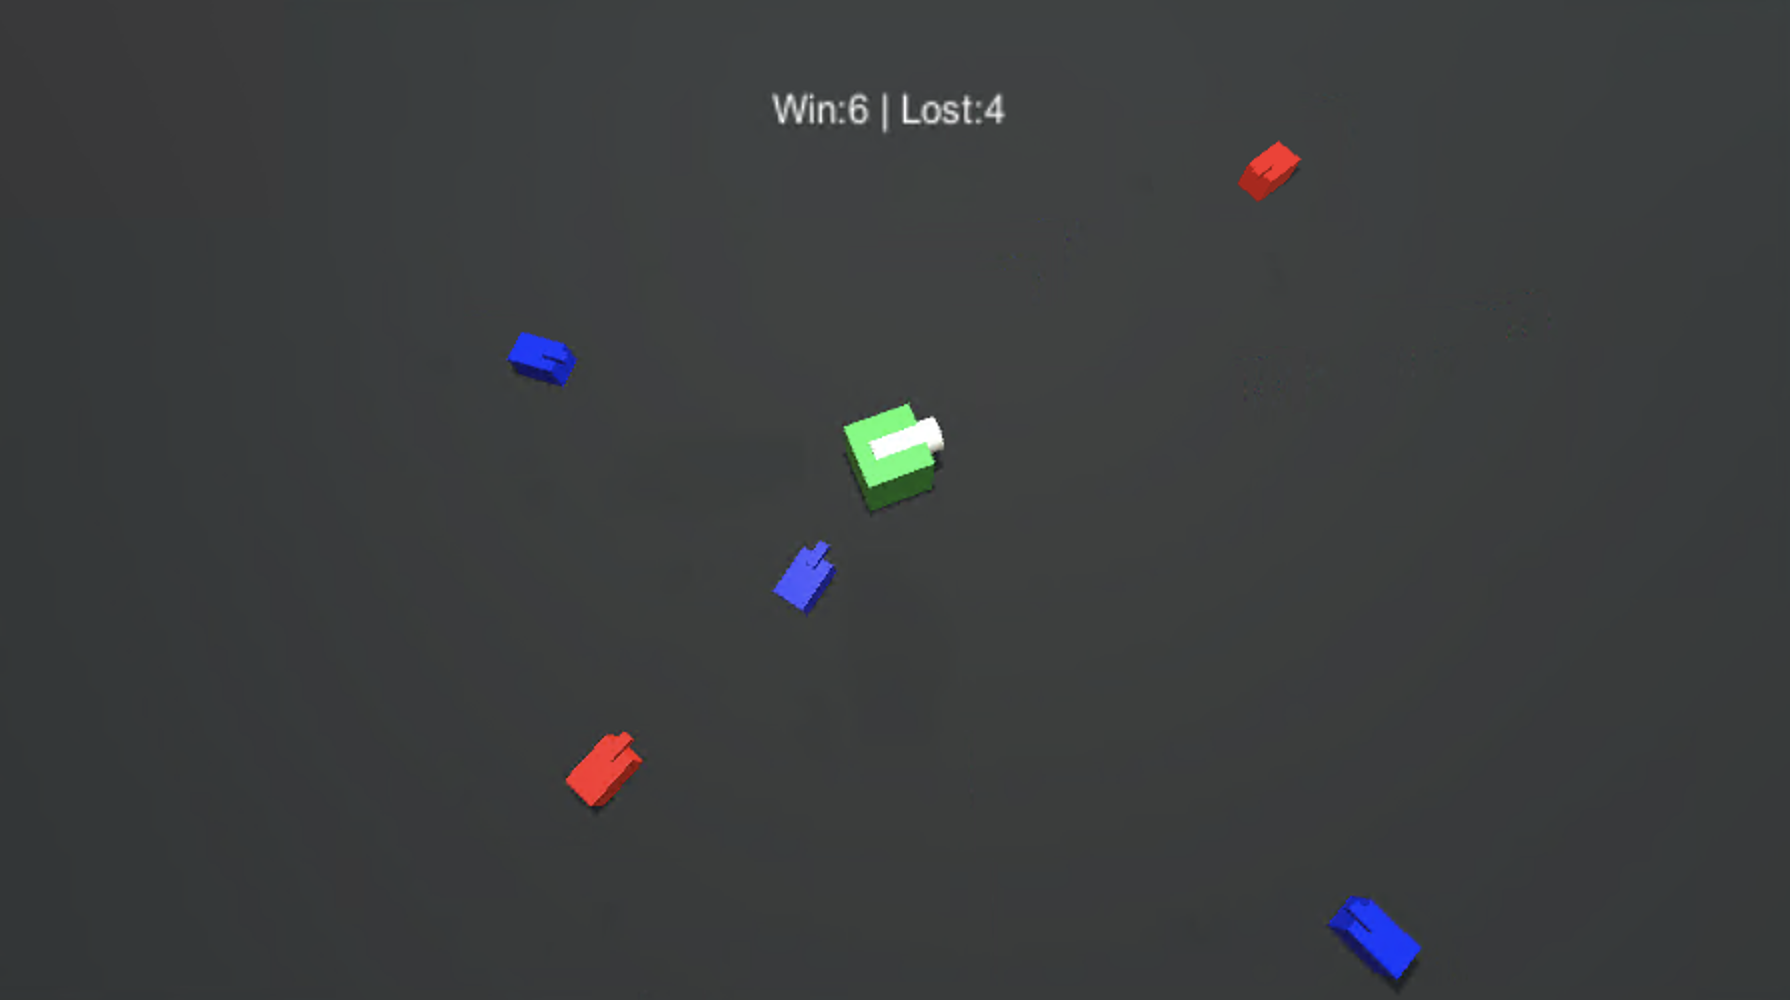
\includegraphics[width=0.5\textwidth]{assets/gameplay_random_spawn}}
\caption{Gameplay from camera view, there units are spawning from random positions, and the scores are updated the episode ends.}
\label{gameplay_random_spawn}
\end{figure}

We added Unity's Textmesh component to display the number of games the agents have won and lost. These scores are placed at the top of the agent and viewed by the camera; it gives us a good idea of how well the agent has performed.

\subsection{Unique points about the game}

Since the turret rotating speed limits its capability, we have provided power-ups to boost rotation speed. The turret gets a temporary boost by shooting a power-up, increasing its rotation by three times for ten seconds. From the reinforcement learning perceptive, we are interested to find out if the agent will go for these power-ups.

Based on the assignment description, both friendly and enemy units has the same movement speed of \textit{2} units. But to make the game more interesting, we set our enemy's movement speed to \textit{3} units in our game design while friendly units are moving at \textit{2} units. We did this right from the start and tested it on the easiest mode. By doing so, it not only made the game more challenging for the agent, but it also allows us to test the agent's priority on shooting enemy units as quickly as possible.

We also introduced advanced enemy in the advanced difficulty, where it would change its direction instead of moving straight into the turret base. Because of its randomness, these enemy units might periodically move faster. These advanced enemies will provide a challenge for the turret agent.

\section{Units}

The purpose of the unit is to move closer to the turret. Units are spawn in a set interval, at a random position around the turret. The configuration determines the distance and how often it will spawn. Each spawned unit will start by facing a random direction. It will rotate to face the turret and move towards the turret. The unit will get saved if it gets closer to the turret.

\subsection{Teams}

A unit can belong to either one of the two teams, friendly and enemy, represented in blue and red, respectively. The unit's team is assigned during its initialization, and the team is critical to determine the game state. Friendly units entering the turret will contribute to the winning condition, while enemy units cause the losing condition to trigger. We assigned a different Unity's \textit{Tag} to friendly and enemy units so that our reinforcement learning agent will be able to learn to recognize them. 

\subsection{States}

At any point in time, each unit will be in one of the four states, 1) \textit{isFree}, 2) \textit{isAlive}, 3) \textit{isHit}, and 4) \textit{isSaved}.

\textit{isFree} state is an inactive unit, where it signifies that this unit's memory space is available to be assigned for new units. This allows us to reuse the same memory for new units, see the memory management section for more information. 

\textit{isAlive} state is an active unit, where it's objective is to move towards the turret regardless of which team this unit belongs to, as their goal is to reach the turret's base. The game controller is able to command these active units to move.

Units that are hit by the turret's ray will change its state from \textit{isAlive} to \textit{isHit} state. At the end of an update cycle, the game controller will check all \textit{isHit} units and increase the respective counters for assessing the end game state. Then after verifying all \textit{isHit} units, the game controller will set these \textit{isHit} units to \textit{isFree} state. This allows us to reuse the same memory for new units.

Units that touched the turret's base will be set to the \textit{isSaved} state. At the end of an update cycle, the game controller will check all \textit{isSaved} units and increment the \textit{units saved} counter for assessing the end game state. Then after verifying all \textit{isSaved} units, the game controller will set these \textit{isSaved} units to \textit{isFree} state.

\subsection{Aesthetics}

As reinforcement learning requires a large volume of gameplay data to learn effectively, we reduced the graphics to improve training by increasing the number of samples gathered per second. Reducing the graphics can dramatically increase the throughput of training samples, allowing us to run with multiple parallel environments concurrently. We use two 3D blocks, one for the body, another block at the top to show where the unit is heading.

\begin{figure}[h]
\centerline{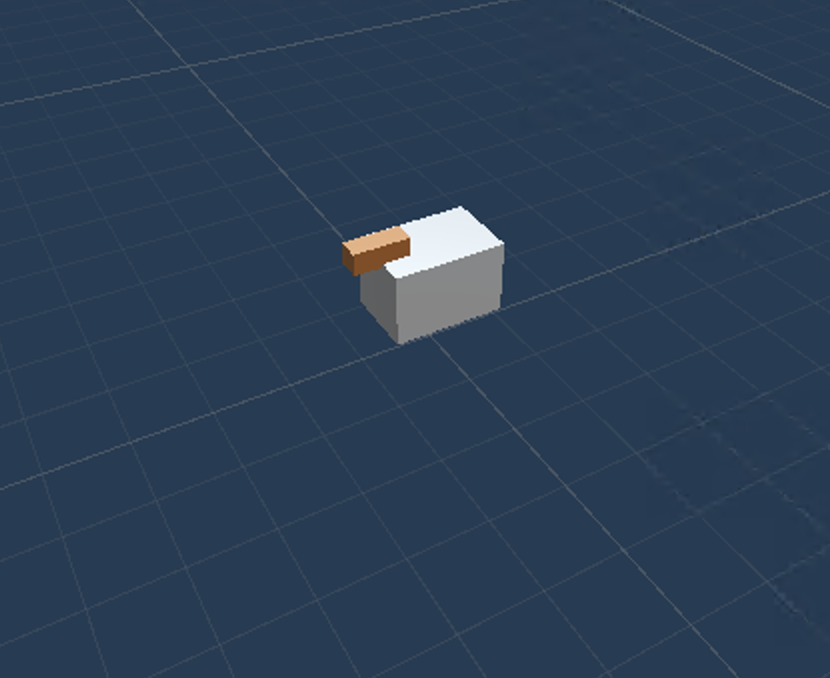
\includegraphics[width=0.5\textwidth]{assets/tank}}
\caption{The basic structure of unit, blue (friendly) or red (enemy) material are assigned during initialization.}
\label{tank}
\end{figure}

\subsection{Movement}

There are two options for the unit's movement, 1) \textit{turn left or right}, and 2) \textit{move forward}. A movement speed parameter limits the forward movement. This parameter is defined during the initialization when the unit is spawned. It can only perform the movement in the \textit{isAlive} state. The game controller triggers the movement of units. At each frame, the unit will check its direction it is currently facing and rotate to face towards the turret. Then, the agent will move forward towards the turret at the assigned movement speed. The move speed of friendly units is \textit{2} units, while the movement speed of enemy units is \textit{3} units. 

\subsection{Custom enemy behavior}

In the advanced difficulty, enemy units can move in a random direction, instead of moving straight for the turret's base. This would cause the turret to waste precious time, spending more time rotating to hit the enemy units. From a reinforcement learning point of view, this could pose a great challenge for the agent as randomness can be difficult to learn and predict. Also, in advanced difficulty, these enemy units can have a random faster movement speed. These fast-moving enemies will pose a more significant threat to the turret agent.

\section{Turret}

The turret is the reinforcement learning agent in the game that we are training. Its objectives are to shoot the enemy units, to prevent them from entering the base while ensuring that friendly units are saved. There are two parameters that we can configure, which limits its performance. Its rotating speed limits the turret, and there is a cool down between each shot. By default, the rotation speed is set to 180 degrees per second, and a 0.75 seconds cooldown between shots.

\subsection{Aesthetics}

Our turret is made up of two game objects, a tower (a cube) and a gun turret (a cylinder). The purpose of the tower is used to determine if units are near enough to be rescued. The gun turret is used to show its current facing direction, where the ray will be fired from.

\begin{figure}[h]
\centerline{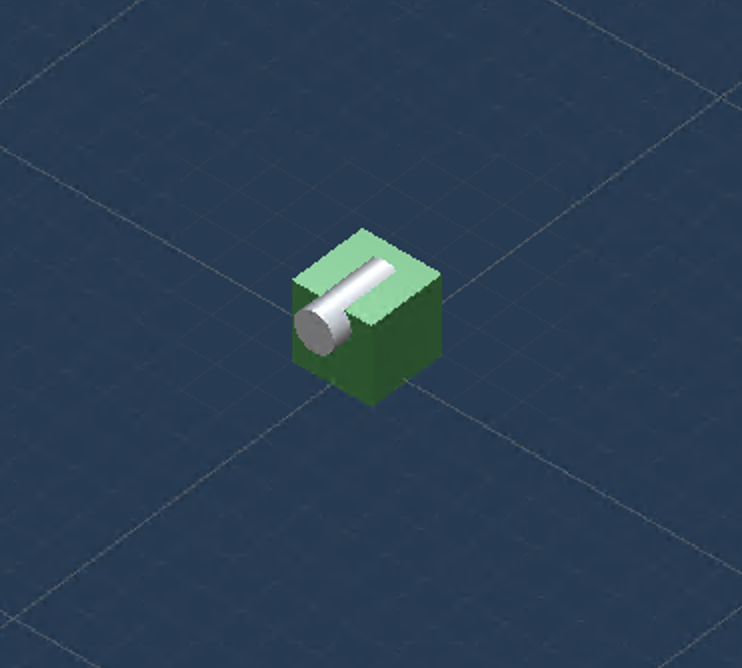
\includegraphics[width=0.5\textwidth]{assets/turret}}
\caption{The basic structure of turret, made up of two game objects, a cube and a cylinder.}
\label{turret}
\end{figure}

\subsection{Controls}

The turret is capable of two actions, 1) \textit{rotate left or right}, and 2) \textit{fire}.

\subsection{Machine Learning Agent Overview}

In the past, non-player character behaviors are hand-coded manually, it is limited, time-consuming, and most of the time, not realistic. From Deep Blue that won the world champion in chess, to AlphaStar to win Grandmaster in StarCraft II, machine learning methods are changing the way we build intelligent AI for gaming. These machine learning methods are changing and solving problems that we never thought were possible. With reinforcement learning, agents learn through interaction in a training environment, where the agent's actions interact directly and change the state of the environment. The agents learn and perform better in the environment over time by providing rewards and punishments.

\subsection{Observations}

Observations are the inputs for our agent to sense the current environment in order to determine the best cause of actions. There are two kinds of observations, parameters-based and sensors.

\subsection{Parameters}

We have two parameters, \textit{ready to fire}, and \textit{time to fire}. \textit{Ready to fire} is a boolean variable for the agent to learn that only when it is \textit{ready to fire} will the shoot action be activated. When the cooldown duration gets larger, this association gets vaguer, poses a challenge for the agent to learn. As such, we introduce another parameter, \textit{time to fire}. We hope this parameter will provide more information on the time left until it is ready to fire.

Initially, we have included the agent's rotation in the Euler angle, but we removed it because where it is currently facing does not determine when the agent should be shooting. This is especially important as we move from static spawn points to random. Including this parameter certainly allow the agent to perform well in the static spawn points scenario, but it performs poorly when the spawn point is random. 

\subsection{Sensors}

Our agent, the turret, receives observations via the Ray Perception Sensor provided by Unity. This sensor sends out a series of ray casts and adds them to the observation stack, which our agent will "see" the environment. These observations are the inputs for the reinforcement learning agent responsible for selecting the best output actions for turning or shooting. 

\begin{figure}[h]
\centerline{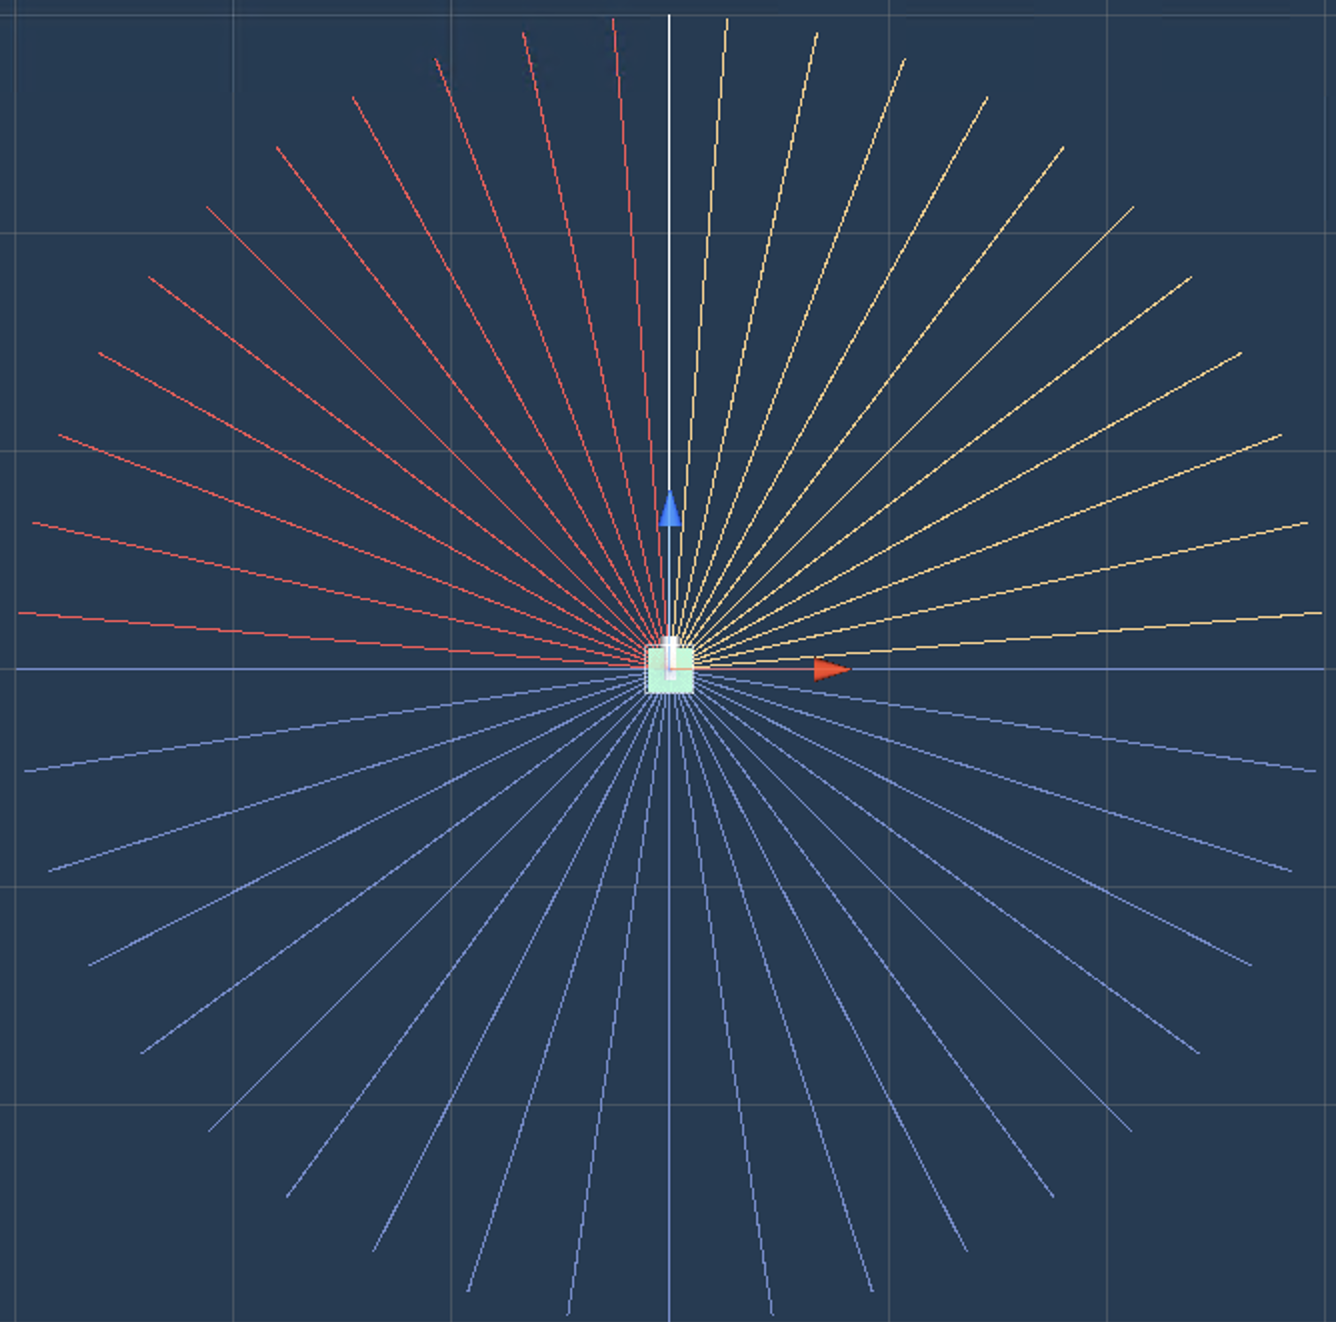
\includegraphics[width=0.5\textwidth]{assets/agent_sensor_2}}
\caption{Ray preception arrangement of the turret. Front sensor (white), left sensor (red), right sensor (yellow), and back sensor (blue).}
\label{agent_sensor}
\end{figure}

We have positioned the Ray Perception sensors to observe 360 degrees around the turret. Each turret are equipped with 4 Ray Perception sensors, \textit{front}, \textit{left}, \textit{right}, and \textit{back}. Each sensor can detect objects up to a distance of 30 units. Fig.~\ref{agent_sensor} shows the agent's ray perception sensors.

\textit{Front}. This sensor has only a single ray, directly in front of the agent. The purpose of this sensor is to aim to associate between target and shooting, acts like hindsight.

\textit{Left}. This sensor has 11 rays, covering 35 degrees on the left of the agent. This sensor aims to allow the agent to sense units on the left, associate detecting units, and turn left.

\textit{Right}. Similar purpose to the \textit{Left} sensor, this sensor covers 35 degrees right of the agent with seven rays.

\textit{Back}. This sensor has 21 rays facing the back of the agent, covering 180 degrees. The purpose of this sensor is to detect units coming from the back of the agent.

\subsection{Rewards}

Reinforcement learning agents take actions to maximize the total cumulative reward. These rewards are signals for the agent if they are performing the task correctly. Likewise, they are punished with negative value rewards if they failed at the task. The agent will score \textit{+10} reward for winning each episode, and \textit{-100} for losing the episode. We reduced the winning rewards because saving friendly and killing enemy units have rewards. 

We designed a reward system to encourage good shooting behavior by reducing the number of missed shots; we introduced a \textit{-1} penalty for missing a unit when firing.

Because of delayed gratification, where we need ten friendly saved before receiving the full reward, we need a way to encourage the agent not to give up. As such, We award \textit{+1} when a friendly unit is saved; this can signal the agent that it is doing something right.

Likewise, due to delayed gratification, we want to encourage the agent to shoot enemy units; thus, we provide rewards for killing enemy units. The reward for killing the enemy decays overtime. Killing the enemy at the maximum distance will reward \textit{+5} points. This reward will reduce as the enemy units move closer to the turret. Thus, when the agent hits an enemy unit, it will get more reward if the enemy is further away than it is closer.

These rewards were tested and implemented over a series of experiments. See the \textit{Review the rewards} section for more details.

\subsection{Parameters}

Table~\ref{table_params} shows the list of parameters for our machine learning. We tune this configuration over 40 iterations and found this suitable for our agent; its mechanism, its observations input, action space, and reward system.

\begin{table}[t]
\centering
\caption{Configuration for reinforcement learning in YAML file.}
\begin{tabular}{c|c}
\hline
\hline
\multicolumn{2}{c}{\textbf{Hyperparameters}} \\ 
batch size & 512 \\
buffer size & 2048 \\
learning rate & 0.0003 \\
beta & 0.01 \\
epsilon & 0.2 \\
lambd & 0.95 \\
num epoch & 50 \\
learning rate schedule & linear \\
\hline
\multicolumn{2}{c}{\textbf{Network settings}} \\ 
normalize & false \\
hidden units & 512 \\
num layers & 2 \\
vis encode type & simple \\
\hline
\multicolumn{2}{c}{\textbf{Reward signals - extrinsic}} \\ 
gamma & 0.99 \\
strength & 1.0 \\
\hline
\multicolumn{2}{c}{\textbf{Reward signals - curiosity}} \\ 
gamma & 0.99 \\
strength & 0.1 \\
encoding size & 256 \\
learning rate & 0.0003 \\
\hline
\hline
\end{tabular}
\label{table_params}
\end{table}

\section{Development and Testing Journey}

We train our agents with 64 parallel environments, generally between 2 million to 10 million steps, on an Intel Core i9 CPU @ 2.80GHz machine. This section detailed the development and testing progress to verify and intensively the difficulty step by step.

\subsection{Test to ensure basic mechanics are working}

In this scenario, our objective is to ensure that the game mechanics are working. As such, we designed a straightforward game to verify each consideration. 

\begin{figure}[h]
\centerline{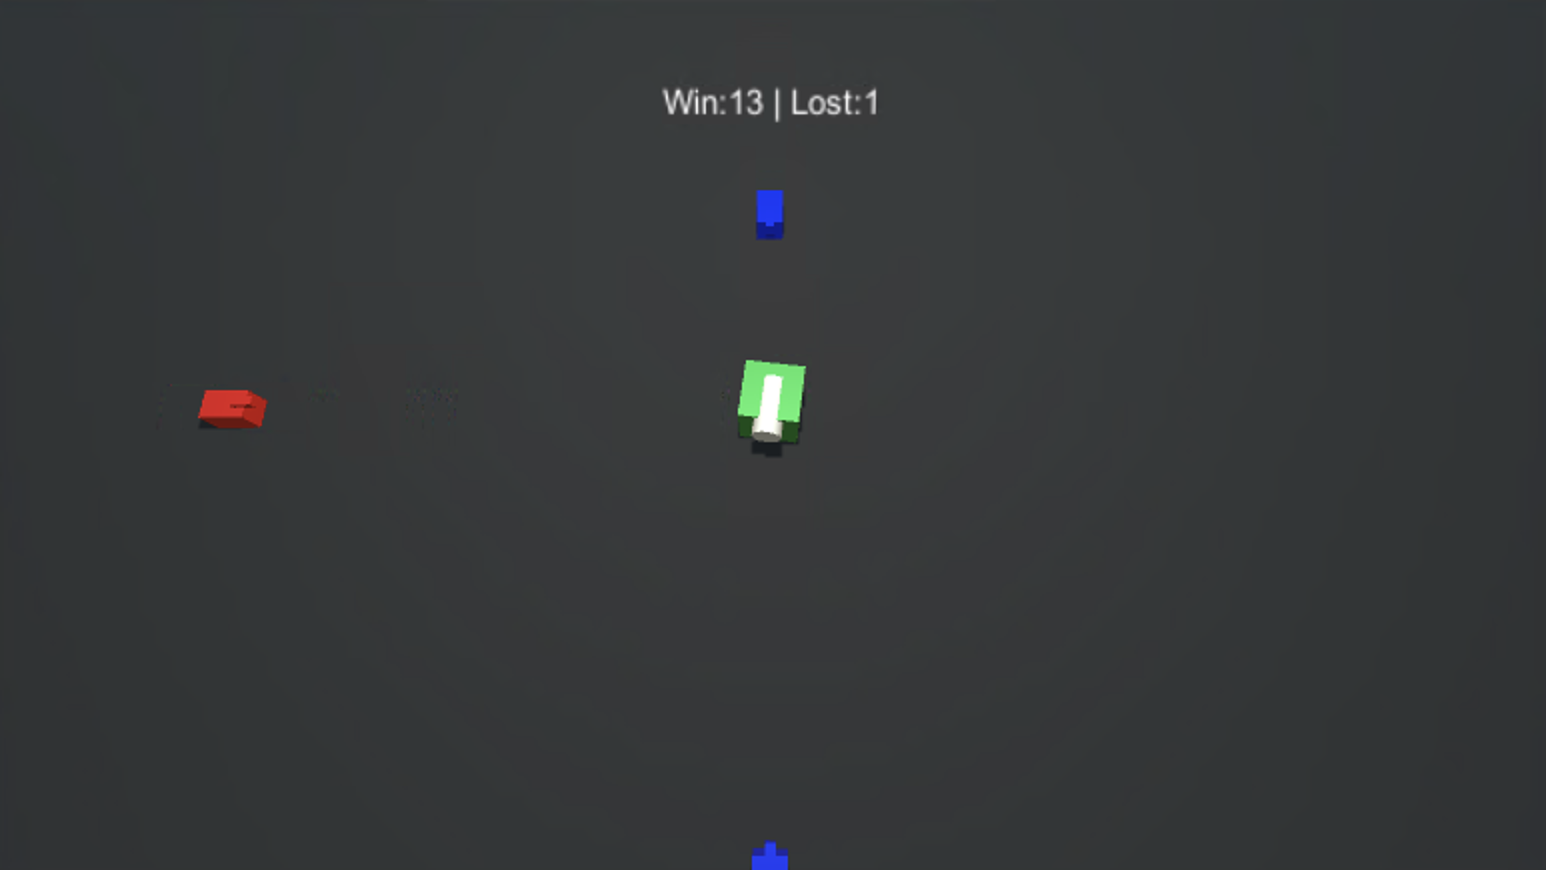
\includegraphics[width=0.5\textwidth]{assets/fixed_spawn}}
\caption{Fixed spawn points where friendly and enemy units will spawn from, but their spawn position will be swapped randomly.}
\label{fixed_spawn}
\end{figure}

Firstly, we want to ensure that the Ray Perception sensor is working, such that it can detect units and its team. We also want to test if Ray Perception can determine distance. This is critical as enemy units that are nearer should be turret's priority. There are four fixed spawn locations in this game mode, north, south, east, and west. Friendly units will be spawned at the north and south, while enemy units in the east and west. Fig.~\ref{fixed_spawn} shows the positions of these fixed spawn points. This will allow us to test the effectiveness of the Ray Perception sensor. During this testing, we detected a bug in our code where, when the ray hit the units, it could hit the unit's parent game object (which contains the unit's component), or it could hit the child game object (that does not have the unit's component). As such, null objects are detected. We did a null check to prevent error logs; although this removes the error logs, it did not solve the problem as turret will often "miss" even though it is a hit. As such, we altered the code to ensure to check both parent and child components. 

Secondly, we wanted to ensure that the actions received from the ML agents are working. While checking the Ray Perception is the input for the agent, we also want to ensure the output actions are correctly implemented. During testing, we realized that our agents only turn in a clockwise direction and do not turn in an anti-clockwise direction. This made us curious and dug deeper. We realized that the discrete values from actions with three spaces are 0, 1, and 2. This is different from our intended design of -1, 0, and 1. This lead to the results where the agents would not receive any \textit{-1} instructions. Thus, they would not be able to turn anti-clockwise. As such, we adjusted the code to be more robust, suitable for both in \textit{heuristic} and in \textit{action received} scenario. Using the \textit{heuristic} function, which is reading from \textit{horizontal} keys, it returns -1, 0 and 1 for turn left, no action and turn right respectively. But this is different from the agents' \textit{action received} function, which is 0, 1 and 2. As such, we will replace \textit{2} with \textit{-1}, which symbolize turning left. In order to ensure that the firing action is working, we remove the fire cooldown in this scenario. This allows us to remove training complications where an action does not yield any results.

\begin{figure*}[ht]
\centerline{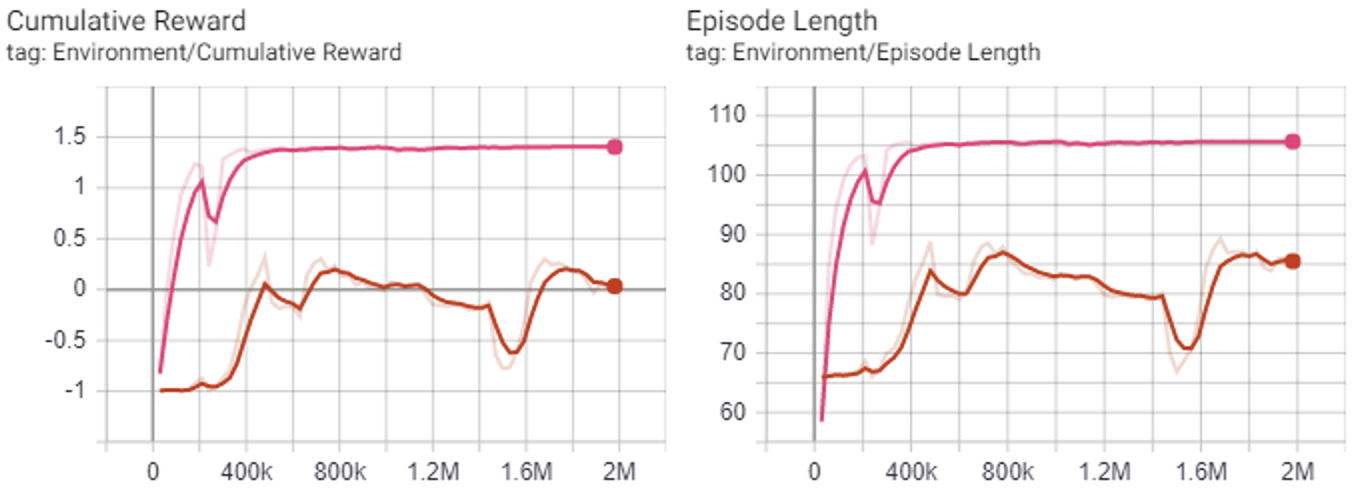
\includegraphics[width=1\textwidth]{assets/scene1_combine_1}}
\caption{Cumulative reward of experiments before (red) and after (pink) fixing game related bugs.}
\label{scene1reward}
\end{figure*}

Fig.~\ref{scene1reward} shows the cumulative reward of the agent before and after these fixes. We trained the agent over 2 million steps, and the agent was able to win all the time after 500,000 steps. To view it in Tensorboard, before the fixes are contain in \textit{run 3}, and after fixes are in \textit{run 4}.

\subsection{Further ensuring ray preception can distinguish friend and foe}

We wanted to know if the turret can distinguish between friendly and enemy units. As such, we changed the win condition to as long as one friendly enters, and the losing condition to one enemy enters or killing one friendly unit. This will allow us to test if the turret can avoid shooting the friendly units. To ensure that the agent can distinguish between the two teams, we swap their spawn points after a random interval. In the previous scenario, we realized that the agent is relying heavily on its facing angle. As such, it was not able to perform at all when the spawn points were swapped. Thus, we removed the facing angle from its observation stack and observed the environment solely relying on the ray perception sensors. Friendly will start by spawning north and south, while the enemy spawns at the east and west. After a random number of episodes, the team will swap their spawn points. We expect the agent to continue to shoot the enemy units. Like previous experience about parent and child component bug, we realized that the units' child components are not tagged (only the parent component containing the unit's code is tagged). Thus, the ray perception only detects friend or enemy tag if it hits the parent component. But because sometimes it hits the child component, and the tag is missing, it fails to learn. As such, we implemented a loop on all it's child components and assign the same tag as the parent. In addition, we removed an input feature that represents the agent's facing direction.

To enhance the ray perception sensor, we added one more sensor to detect what the agent is facing, with 10 degrees view angle and six rays. We do this to enhance the agent's detection, so that agent might only shoot if this sensor detects the correct target. This was later removed to reduce input complexity.

\begin{figure*}[ht]
\centerline{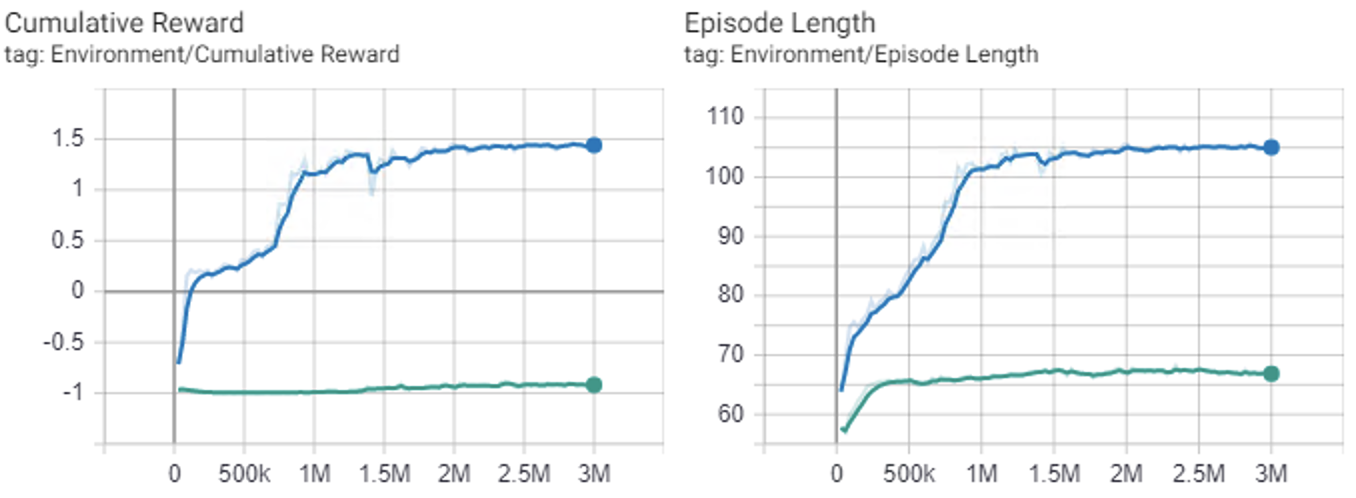
\includegraphics[width=1\textwidth]{assets/scene2_combine_1}}
\caption{After introducing random swap spawn points, the cumulative reward of experiments of before (green) and after (blue) fixing ray preception related bugs.}
\label{scene2reward}
\end{figure*}

Before these fixes, as the spawn points were swapped randomly, the agent performed poorly. Fig.~\ref{scene2reward} shows the cumulative reward of the agent before and after these fixes. We trained the agent over 3 million steps, and the agent was able to achieve a 100% win rate after 1 million training steps. To view it in Tensorboard, before the fixes are contain in \textit{run 6}, and after fixes are in \textit{run 9}.

\subsection{Test delayed gratification}

It is challenging for reinforcement learning agents to learn good and bad actions if the rewards are delayed. This requires a certain level of long-term planning in order for an agent to learn how to maximize returns, as opposed to an immediate reward. So far, our agent's objective was to save one friendly unit from winning the game; increasing the number of units needed to save will result in delayed rewards.

\begin{figure*}[ht]
\centerline{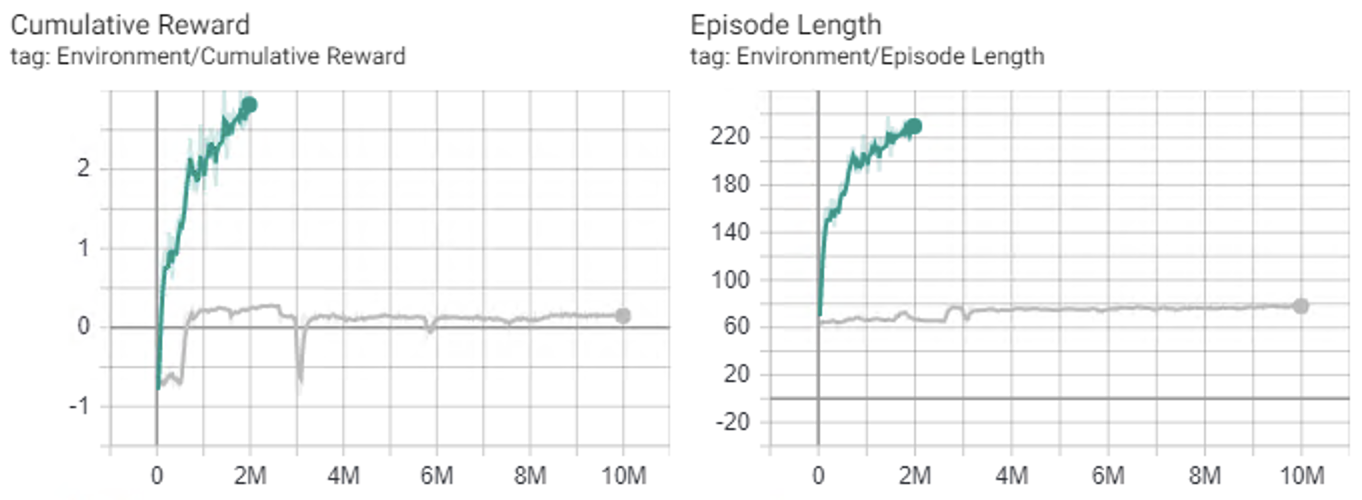
\includegraphics[width=1\textwidth]{assets/delayed_gratification}}
\caption{Cumulative reward of experiments of before (grey) and after (green) including mini-reward for shooting a target. Before, the agent fail to learn despite after 10 million training steps.}
\label{delayed_gratification}
\end{figure*}

To test delayed gratification, we increased the win conditions to saving ten friendly units. As expected, the agent could not learn as it will receive a negative reward before it has the chance to save ten friendly units. In the end, the agent simply stopped shooting, as shooting the enemy does not yield any points, while shooting a friendly unit results in immediate failure. It is safer not to shoot and has allowed the enemy into the safe zone. As such, we want to encourage turret to shoot units. Thus, we reward for each target hit. But shooting a friendly unit will result in immediate failure, this will encourage the turret not to hit the friendly units. 

Fig.~\ref{delayed_gratification} shows the cumulative reward of the agent with and without the reward for hitting the target. We observed that, even after training for 10 million steps, the agent failed to learn the game, and every episode lasted for the same duration. But with the mini-reward for shooting enemy units in place, after training the agent over 2 million steps, the agent was able to nail the game. 

\subsection{Random spawn points}

Unlike fixing spawn points, random spawn points will result in cases when a friendly unit is protecting enemy units by following a friendly unit. Fig.~\ref{scene_gameplay_random_spawn} shows a snapshot of units appearing from random spawn points. Having random spawn points are much more unpredictable; the agents might not have the chance to learn anything. Due to the difficultly of delayed gratification and random spawn points, we trained our agent over 20 million steps, to view the training progress in Tensorboard, see \textit{run 18}. Despite the long training duration, there are many poor performance experiments, which led us to investigate in detail. The next few sections describe how we debug and improve its performance.

\subsection{Review the rewards}

So far, our rewards system has been very straightforward, \textit{+1} for winning (saving ten friendly units), and \textit{-1} for losing (killing a friendly or letting one enemy in). What we realized is, for some reason, the agent will only fire only when the enemy units get really close. As such, we developed a new reward system. We reward the agent for every enemy shot, and that reward decays overtime. When the agent hits an enemy unit, it will get more reward if the enemy is further away than it is closer. We hope that our agent will prioritize and take more risks to shoot enemies further with this new design. Because rewards are given for killing enemy units, we increase the winning reward to \textit{+10} and \textit{-10} for losing the episode. 

However, after including rewards for killing enemy units, the unexpected result was that the agent ended the game early by killing friendly units. Our hypothesis is that the agents are getting more points from killing enemy units than from winning the game. As such, we increased the penalty for losing to \textit{-100} while maintaining \textit{+10} for winning. Asa result, our agent prioritizes on winning the game, and the result of this change is recorded in the \textit{Results} sections.

\subsection{Raycast size}

We have been using the Raycast to fire at units. After much inspection, we realized that the hitbox of Raycast is much smaller than our \textit{Front} Ray Perception. This caused a technical issue as the front sensor detected a unit, but the firing mechanism did not hit any target. Therefore, we replaced \textit{Raycast} to \textit{SphereCast}, where it allow us to specify the size of the hitbox. We tested this configuration on advanced difficulty, and our agent was finally able to perform. We trained the agent for 10 million steps, Fig.~\ref{run_21} shows the agent's cumulative reward after this fix.

\begin{figure*}[ht]
\centerline{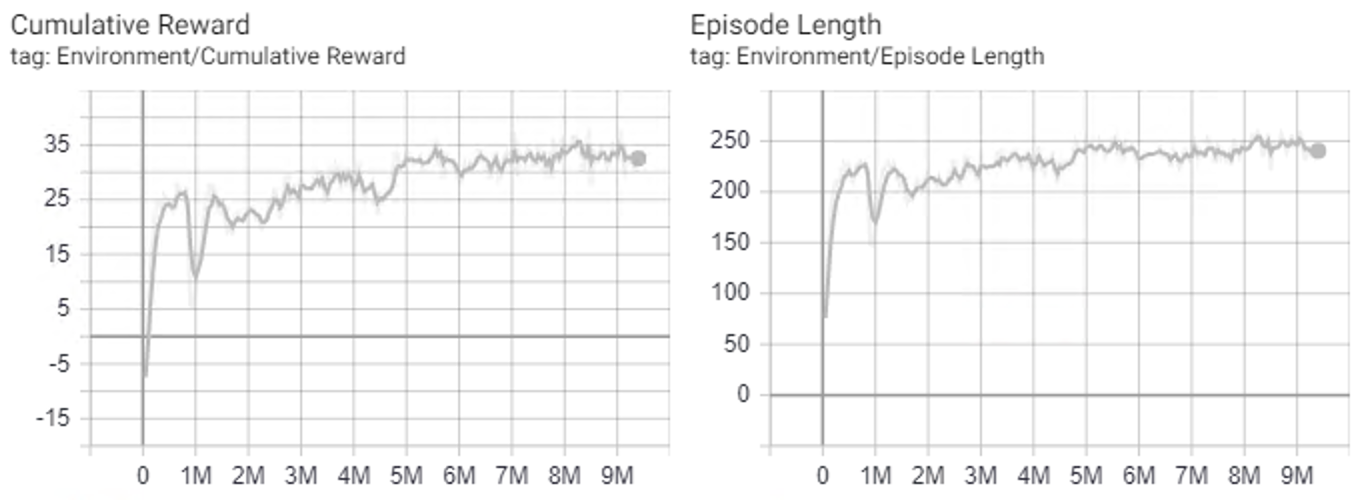
\includegraphics[width=1\textwidth]{assets/run_21}}
\caption{Cumulative reward after matching the Raycast size with Ray Perception.}
\label{run_21}
\end{figure*}

\section{Results}

We train and test our agents by running in parallel, 64 simulated environments. After executing more than 40 experiments (Tensorboard to see each run, and failed runs are replaced), in order to balance between training time and performance, we train our agents for each scenario for 2 million steps. Lastly, we benchmark each experiment with the win rate in 1,000 episodes. Table~\ref{table_results_winrate} shows the win rate for each experiments. Fig.~\ref{all_runs_final} shows the cumulative reward of all the final experiments for each scenario during training. Based on our current reward systems, the possible cumulative rewards range is approximately from \textit{-100} to \textit{+100}.

\begin{table}[t]
\centering
\caption{Performance for each scenario.}
\begin{tabular}{||c|c|c||}
\hline
\textbf{Scenario} & \textbf{\% winrate in 1000 episodes} \\
\hline
Easy & 99\% \\
\hline
Normal & 83\% \\
Normal with power-up & 65\% \\
\hline
Advanced & 57\% \\
Advanced with power-up & 56\% \\
\hline
\end{tabular}
\label{table_results_winrate}
\end{table}

\begin{figure*}[ht]
\centerline{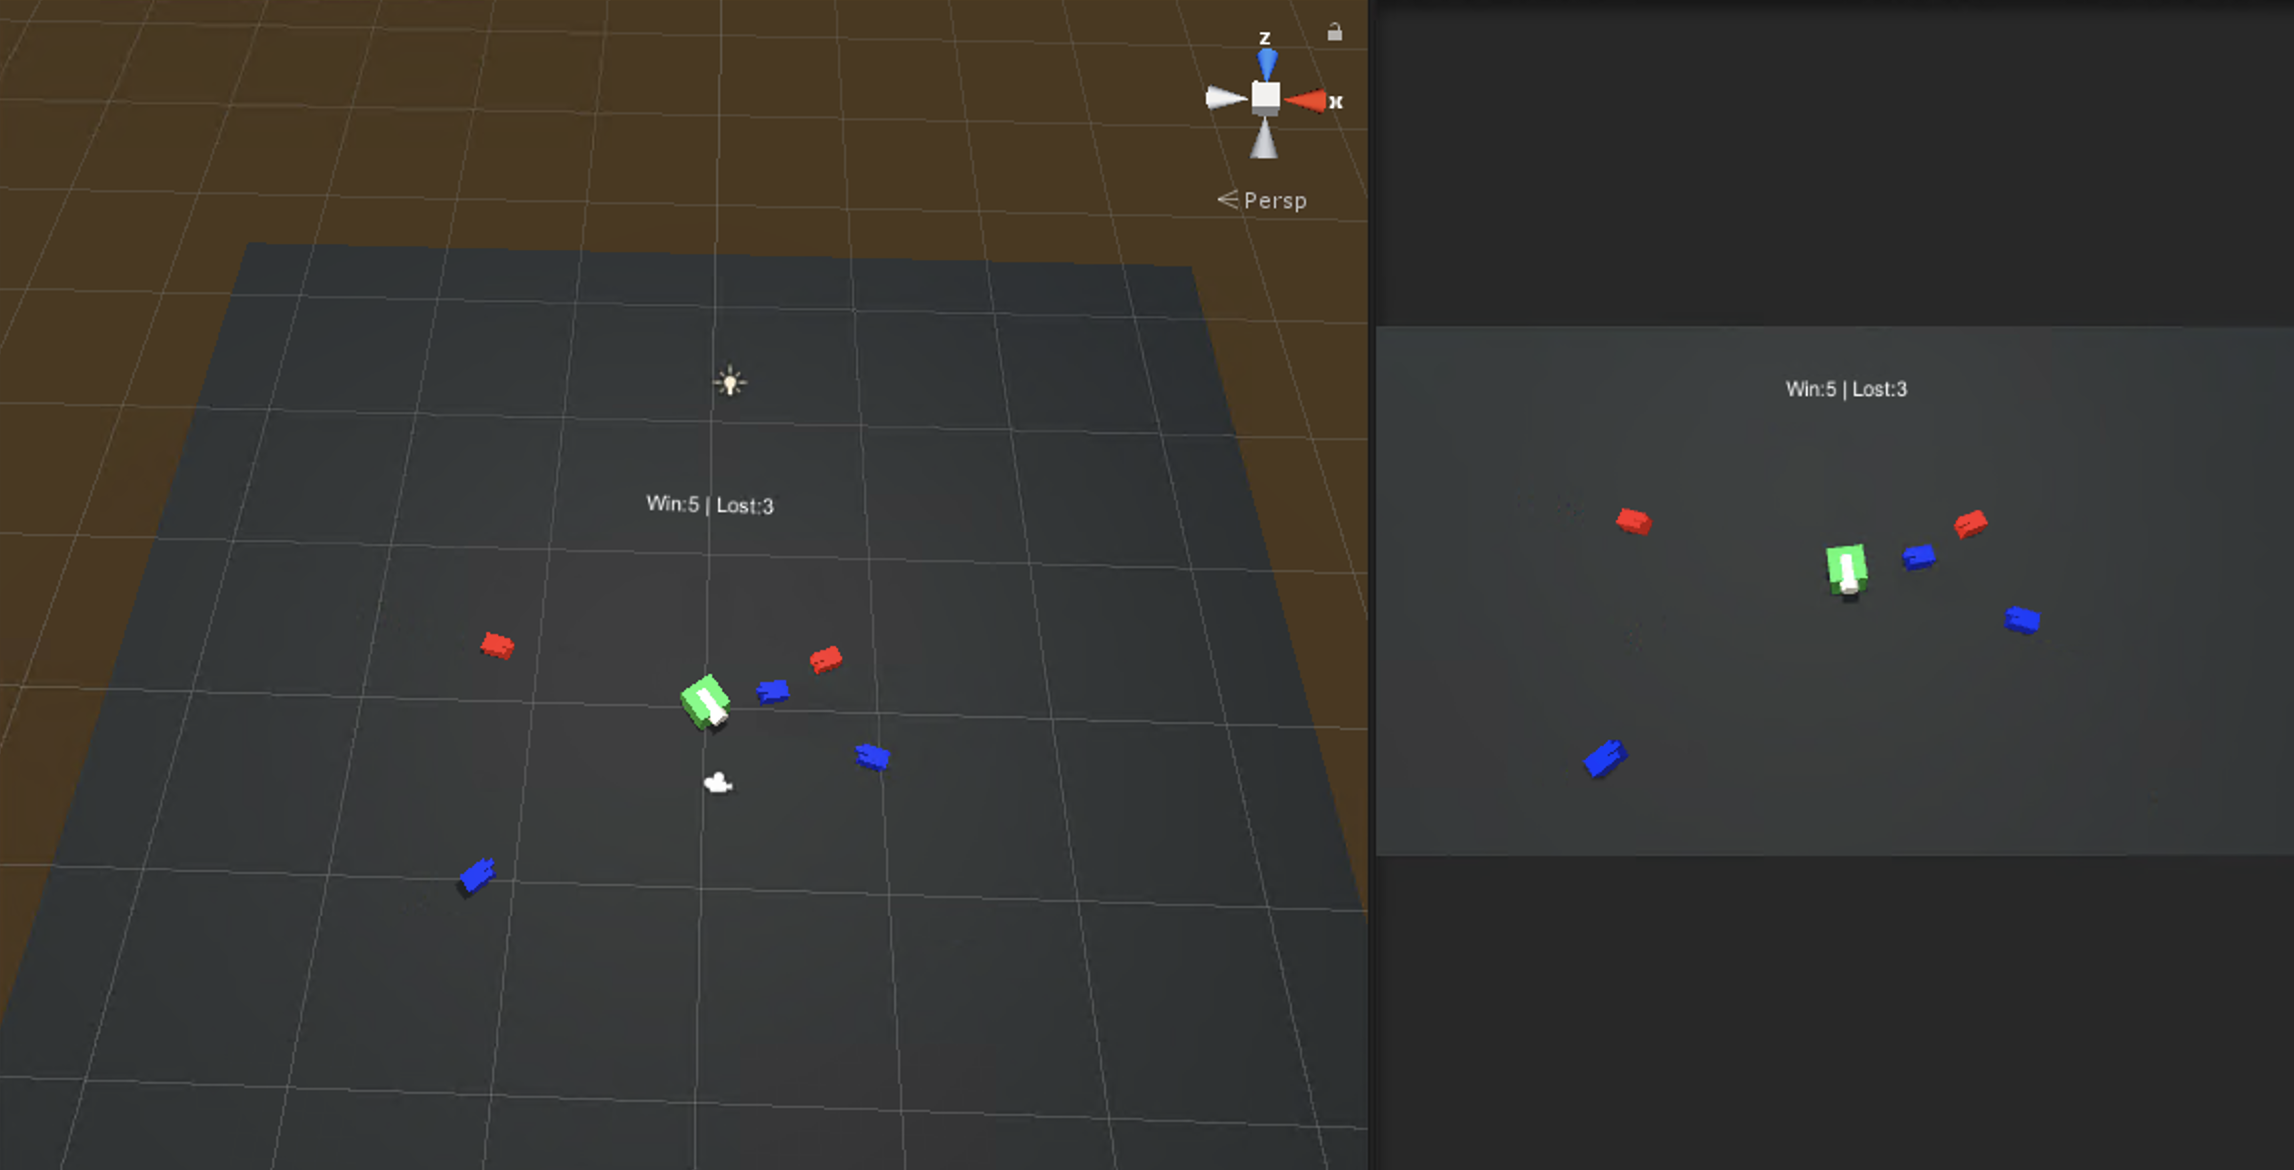
\includegraphics[width=1\textwidth]{assets/gameplay_unity_random_spawn}}
\caption{A snapshot of the gameplay, visit the companion website to watch the gameplay video.}
\label{scene_gameplay_random_spawn}
\end{figure*}

\begin{figure*}[ht]
\centerline{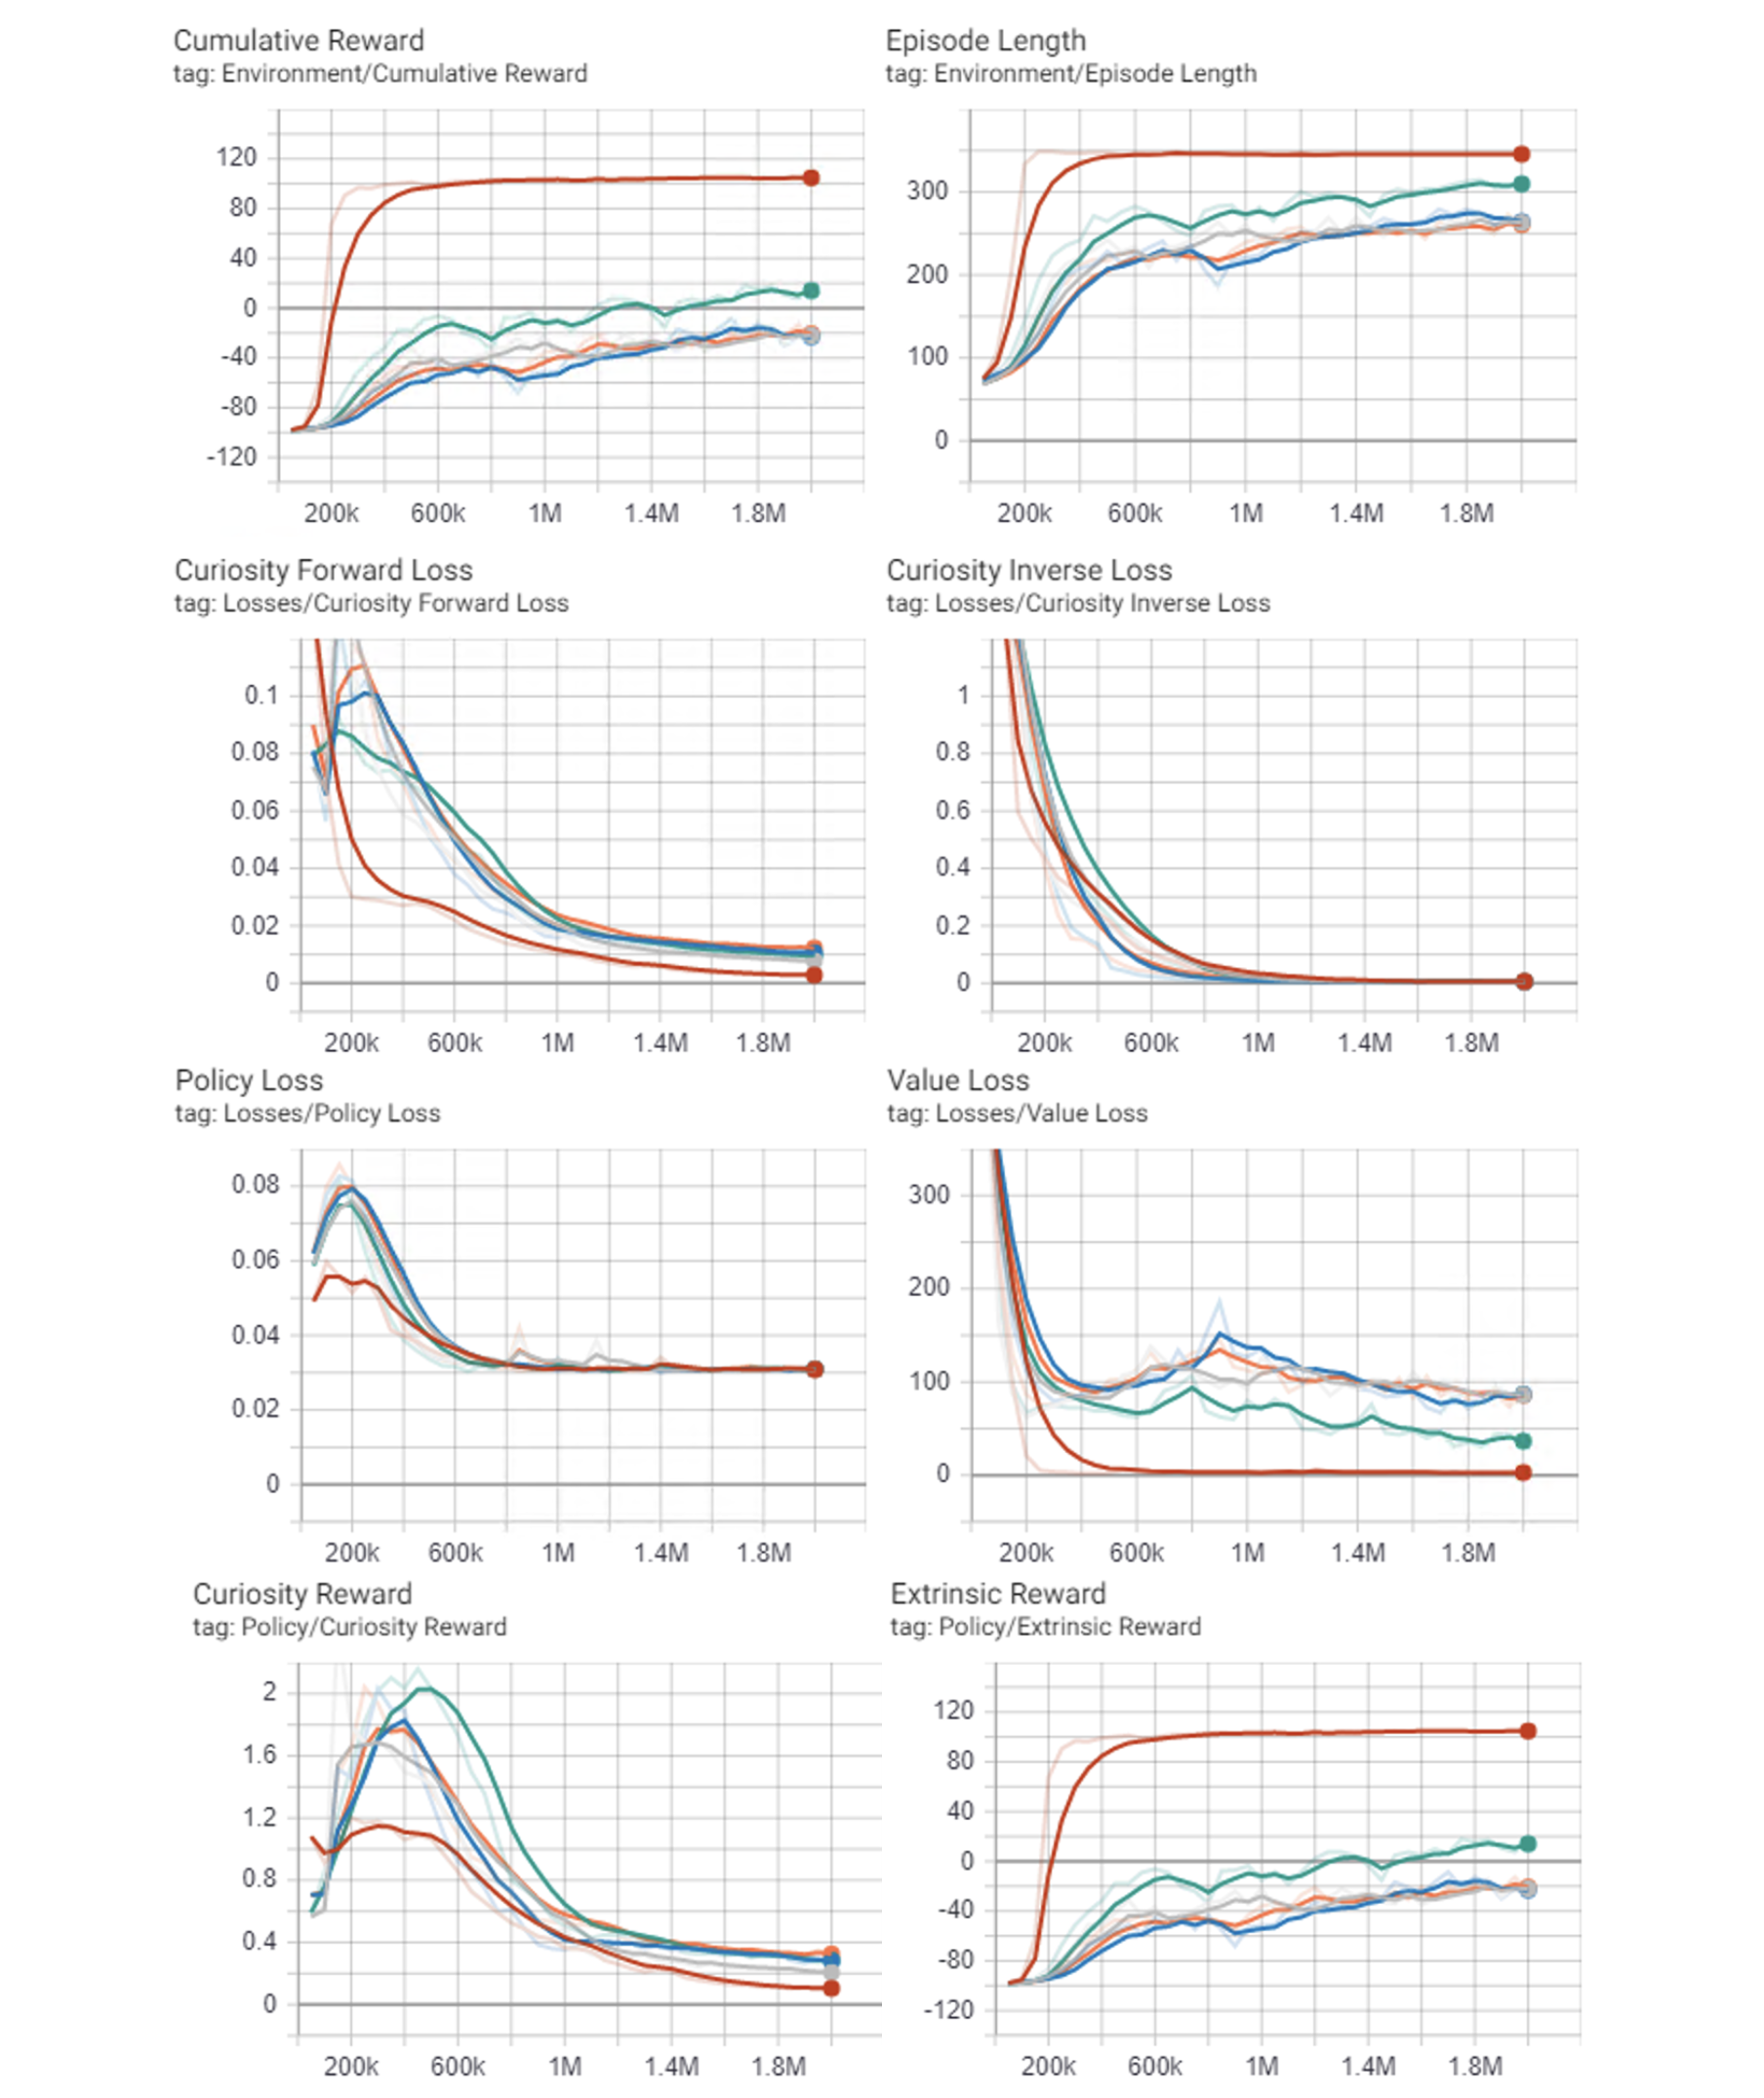
\includegraphics[width=1\textwidth]{assets/all_runs_final}}
\caption{Showing metric for each scenario shown on Tensorboard. Easy (red), Normal (green), Advanced (grey), Normal with power-ups (orange), and Advance with power-ups (blue).}
\label{all_runs_final}
\end{figure*}

\subsection{Performance of the AI at the easiest level}

This scenario is where there are fixed spawn points for units, where the friendly and enemy spawn points are swapped at a random interval. Here we test the effects of delayed gratification where the agents are required to save ten friendly units from getting the reward. As this scenario is easy enough, the performance is astounding, with an almost 99\% win rate. Out of 1000 episodes, there are five losses, all of which only happened in the first episode. 

This scenario is particularly important as it proves that the agent was able to distinguish between friendly and enemy units and was able to prioritize shooting nearer enemy units first. With these results, we are ready to challenge our agent to a slightly more difficult scenario.

\subsection{Performance of the AI on the normal scenario}

This scenario is based on the assignment description and requirements, where units are spawned randomly at a specified distance at a specified time interval. Instead of having the same movement speed for both friendly and enemy, we made the enemy faster. This gives a good challenge for our agent. There are so many iterations before the agent manages to learn to play this scenario, see the \textit{Development and Testing Journey} section.

Out of the 1000 episodes, our agent won approximately 83\% of the time. Fig.~\ref{scene_gameplay_random_spawn} shows a snapshot of the gameplay. Visit the companion website\footnote{\href{https://github.com/jinglescode/unity-ml-agents-turret-defense}{github.com/jinglescode/unity-ml-agents-turret-defense}} to watch the gameplay video and source code. 

In most cases, where the agent failed, the enemy is behind a friendly unit, and as the enemy moves faster than the friendly unit, this would result in certain failure. We also notice that the rotation speed has limited the agent's performance, as turning towards an incoming unit from behind, especially enemy units that sneak behind a friendly unit; this would result in a lost episode. Also, in many cases, enemy units are too close to a friendly unit. As a result, shooting friendly units caused the agent to lose the match. One possible way to improve is to fine-tune the size of ray perception and the ray cast. 

\subsection{Performance of the AI on the advanced difficulty scenario}

As in our design, enemy units are already moving faster than friendly units, with advanced enemy units, their movement speed is much more unpredictable. They could move forward faster and move left or right, hiding behind friendly units. This gives a great challenge for our agent; the winning rate is approximate 55\%. Like the normal scenario, there are many cases when the enemy units are hiding behind friendly units; this caused the enemy units to be too near before the agent had the chance to shoot it. At times, the enemy units were moving too close to friendly units. As a result, friendly fire happened, and the match was lost.

\subsection{Performance of the AI with power-ups}

In this scenario, we are interested in seeing the effects on power-ups to see if it improves the agent's performance. The agent gained three times on rotation speed boost and no cooldown on firing by shooting on the power-up. Unfortunately, the performance did not improve. We hypothesize that the agent did not manage to associate shooting the power-ups with the rewards gain as we did not assign any rewards for hitting the power-ups. Therefore, we attempted to assign a small reward for shooting the power-ups. Unfortunately, we did not see any improvements as well.

\section{Conclusion}

This assignment has allowed us to experience and experiment with designing reinforcement learning to perform a task. It is interesting to see that, without handcrafting any rules for the agents, it figures out the game's mechanism by exploring the game. We can see that there are many components to a successful reinforcement learning agent, with a functioning game mechanism, proper usage of observation and action space, and well-designed rewards systems; these contribute largely to its success. 

For additional materials and assets used in this report can be found on Github (\href{https://github.com/jinglescode/unity-ml-agents-turret-defense}{github.com/jinglescode/unity-ml-agents-turret-defense}). The source code can be found in the ml-agents branch (\href{https://github.com/jinglescode/unity-ml-agents-turret-defense/tree/ml-agents}{github.com/jinglescode/unity-ml-agents-turret-defense/tree/ml-agents}).

\end{document}
